\documentclass{kththesis}

\usepackage{blindtext} % This is just to get some nonsense text in this template, can be safely removed
\usepackage{multirow}
\usepackage{graphicx}

\usepackage{csquotes} % Recommended by biblatex
\usepackage{biblatex}
\addbibresource{references.bib} % The file containing our references, in BibTeX format


\title{Feature Selection Methods for Classification of Breast Cancer}
\alttitle{Attributurvalsmetoder för klassificering av bröstcancer}
\author{Niklas Lindqvist\newline Thony Price}
\email{nlinq@kth.se\newline thonyp@kth.se}
\supervisor{Pawel Herman}
\examiner{Orjan Ekeberg}
\programme{Degree Project in Computer Science}
\school{School of Computer Science and Communication}
\date{\today}


\begin{document}

% Frontmatter includes the titlepage, abstracts and table-of-contents
\frontmatter

\titlepage

\begin{abstract}
  >> This will be written later on...

  \blindtext
\end{abstract}


\begin{otherlanguage}{swedish}
  \begin{abstract}

    >> This will be written later on...

    Träutensilierna i ett tryckeri äro ingalunda en oviktig faktor,
    för trevnadens, ordningens och ekonomiens upprätthållande, och
    dock är det icke sällan som sorgliga erfarenheter göras på grund
    af det oförstånd med hvilket kaster, formbräden och regaler
    tillverkas och försäljas Kaster som äro dåligt hopkomna och af
    otillräckligt.
  \end{abstract}
\end{otherlanguage}


\tableofcontents


% Mainmatter is where the actual contents of the thesis goes
\mainmatter


\chapter{Introduction}

% We use the \emph{biblatex} package to handle our references.  We therefore use the command \texttt{parencite} to get a reference in parenthesis, like this \parencite{heisenberg2015}.  It is also possible to include the author as part of the sentence using \texttt{textcite}, like talking about the work of \textcite{einstein2016}.

%add a comment about FNA and RNA data?



Breast cancer is a disease of major concern and is the leading cause of cancer deaths among women \parencite{althuis2005}. At present there are no effective ways to prevent breast cancer. However, efficient diagnosis in an early stage can increase the chance of full recovery. This makes early detection and diagnosis an important issue and screening mammography is the primary imaging modality for early detection of breast cancer \parencite{tabar2001}.

Hospitals today are well equipped with data collection devices to do monitoring and data such as mammography screenings can be collected and shared in information systems. The data can be used by medical personnel to increase their understanding of different diseases. The data can also be used in computer aided diagnostic (CAD) where machine learning algorithms enable tools for intelligent data analysis. CAD makes use of machine learning techniques that learn a hypothesis, a statistical prediction about a patient's diagnosis from a large set of previously diagnosed examples.  The overarching purpose is to assist medical experts in more efficient and accurate diagnostics \parencite{li2007}. Machine learning algorithms is a well studied field within medical diagnosis and well suited for analyzing medical data especially within small specialized diagnostic problems such as breast cancer \parencite{kononenko2001}.

Multiple studies of CAD on breast cancer have been conducted, primarily focusing on classifying mammography data as malignant or not, such those of \textcite{ramos2012} and \textcite{akay2009}. The act of feature selection, removing redundant or irrelevant features from a dataset, can provide classifiers to be faster, more cost-effective and accurate [8]. It is also explicitly mentioned as a topic in need of more research in studies on breast cancer diagnostics \parencite{akin2011}.

\section{Research Question}

In our thesis we will study the impact of different feature selection methods on the classification rate of malignant breast cancer by different machine learning methods. We aim to answer the following:

\begin{itemize}
  \item Does the feature selection improve the accuracy of classification compared to using all features?
  \item In which machine learning methods does feature selection have the greatest impact?
  \item What features are most important for accurate classification of breast cancer?
\end{itemize}

Our hypothesis is that overall the feature selection will improve the classification rate of the machine learning methods used in the context of breast cancer classification. This hypothesis is based on previous research reported by \textcite{karabulut2012}, where it was found that classification accuracy on 15 different datasets was increased by the use of filter methods for feature selection.

Our research differs from the work presented in \parencite{karabulut2012} in the amount of datasets used and amount of classification methods. In our project we will put more emphasis on breast cancer using only datasets of that type. The previous work only investigated feature selection methods by filtering which we will extend by implementing wrapper methods. Lastly, the research scope in this thesis includes a study of the effect of different feature selection methods on Support Vector Machines (SVM), which was not discussed by \parencite{karabulut2012}.

\section{Approach}

Trials will be conducted with feature selection Wrapper methods and feature selection Filter methods. The result of the feature selection methods will be used with different classifiers to evaluate their performance. To broaden the base for comparison we use classifiers from different disciplines, Decision Tree (Logic Based Algorithms), ANN (Perceptron-Based Techniques), Naive Bayes (Statistical Learning Algorithms) and SVM (Support Vector Machines) \parencite{wallace2007}. Feature selection methods and classifiers are denoted in table \ref{table:methods}.

\begin{table}[ht]
\begin{center}
\begin{tabular}{ |l|l| }
\hline
\multicolumn{2}{ |c| }{\textbf{Implementations}} \\
\hline
\multirow{4}{*}{Classifiers}
 & Decision Tree \\
 & Support Vector Machine \\
 & Probabilistic Method \\
 & Artificial Neural Network \\ \hline
\multirow{2}{*}{Feature Selection by Wrapping}
 & Recursive Feature Elimination (RFE) \\
 & Sequential Feature Selector (SFS) \\ \hline
\multirow{2}{*}{Feature Selection by Filter}
 & Chi-square \\
 & Entropy \\
\hline
\end{tabular}
\caption{All classifiers should be tested with each feature selection method.}
\label{table:methods}
\end{center}
\end{table}

A comparison of the classification rate on the machine learning methods without any feature selection and with feature selection will be conducted in order to establish the importance of feature selection in different machine learning approaches when classifying breast cancer. The evaluation criteria will primary be F1 score that conveys the balance between recall and precision of classification performance \parencite{muc1992}. Secondly, we will compare computational resources of the learning phase measured in time. The Breast Cancer Wisconsin (Diagnostic) dataset \parencite{dua:2017}, contains 569 instances with 32 attributes describing the features of breast cancer. Each instance is classified as benign (357) or malignant (212).

\section{Outline} %add chapter 5 and 6

In the Background section earlier work on the topic will be more thoroughly presented on order to clarify how this thesis relates to the field. The following chapter, Methods will detail the methods used to achieve the results that are presented in chapter 4.

\chapter{Background}

\section{Computer Aided Diagnostics}

Machine learning techniques have been successfully applied to computer-aided diagnosis where it by a computerized procedure provides a second objective opinion for the assistance of medical image interpretation and diagnosis \parencite{li2007}, \parencite{ni2016}. To make a CAD system samples with diagnosis i used for learning. In the case of breast cancer diagnosis a radiologist label scans which then can be used to learn a hypothesis whether a undiagnosed sample is benign or malignant cancer \parencite{li2007}.

\section{Breast Cancer} %add Fine needle aspiration in this chapter?

A study in Sweden by \textcite{tabar2001} found breast carcinoma mortality was reduced by 63\% after mammography was introduced. This clearly emphasize the benefits of screening which had resulted in a increased usage of the method to detect and diagnose breast cancer. The increasing demand for mammography image interpretation lead to a shortage of medical radiologist to perform this task and consequently non medical personnel supplement the mammography image interpretation (MII) \parencite{culpan2016}. As breast cancer continues to be the leading cause of cancer mortality among women and more efficient diagnostics and pathology is high on demand the need of low-cost point-of-care is very much needed as stated by \textcite{martei2018}.\\

Fine needle aspiration (FNA) is a diagnostic tool to aspirate cell samples by sampling cells, staining them and examine under a microscope \parencite{FNA}. An example of such sample can be seen in \ref{fig:fna_nuclei}. The cell samples can be evaluated within 24 hours and the method is cost-effective and can be used as a preoperative tool for investigation of tumors. The method is also complication-free and has been widely used for the past 60 years.

\begin{figure}[ht!]
  \centering
  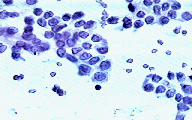
\includegraphics[]{images/fna_nuclei.png}
  \caption{Image caption and source of image goes here? See link in LaTeX comments.}
  \label{fig:fna_nuclei}
\end{figure}

% http://webcache.googleusercontent.com/search?q=cache:635J2rrIdWsJ:pages.cs.wisc.edu/~olvi/uwmp/cancer.html+&cd=1&hl=sv&ct=clnk&gl=se

\section{Feature Selection}

The benefits of selecting a subset of all available features are manyfold, among other it facilitates data visualization and data understanding, reduces the measurement and storage requirements and reduces training and utilization times. In cases with thousands of features it is essential to work with a subset of the data to produce results. \parencite{guyon2003}.

\subsection{Filter methods}

Filters evaluate each feature independent from the classifier, rank the features after evaluation and take the superior ones. The evaluation can be performed by many methods such as Information Gain and Variance \parencite{guyon2003}.

\subsection{Wrapper methods}

Wrappers utilize the learning machine of interest as a black box to score subsets of variable according to their predictive power \parencite{guyon2003}. The issue is as datasets become very large this method might be overly computational intense as finding the optimal subset is considered to be NP-hard \parencite{amaldi1998}.

\section{Related Work}

The paper Discovering Mammography-based Machine Learning Classifiers for Breast Cancer Diagnosis \parencite{ramos2012} uses 20,000 machine learning classification configurations to evaluated their ability to correctly classify malignant cancer. They built a database containing 286 cases and found classifiers that scored with an area of 0.996 under the Receiver operating characteristic (ROC) curve.



In 2011 a study by Akin Ozcift and Arif Gulten \parencite{akin2011} demonstrated that ensemble learning can be used in computer aided diagnostics (CAD) to improve the performance of rotation forest classifier. Using three different dataset and 30 classifying algorithms the average accuracy improved on all datasets. The datasets and their improvement were:

\begin{itemize}
  \item Diabetes: improvement of 2.32\%
  \item Heart diseases: improvement of 2.97\%
  \item Parkinson's: improvement of 2.7\%
\end{itemize}

The improved accuracy demonstrates the effect of feature selection on classification accuracy.\\

Abdel-Ilah and {\v{S}}ahinbegovi{\'{c}} \parencite{Abdel-Ilah2017} used the Wisconsin breast cancer database to investigate the optimal number of hidden layers and neurons for a feed forward back propagation network (FFBPN). Using three different transfer functions: Logsig, Tansig and Pureline. The highest accuracy was 98\% using 3 hidden layers and 21 neurons. Suggestion was made to further investigate different parameters of ANNs to find their effect on the dataset.

\textcite{akay2009} investigated the performance of classification of a SVM with a RBF kernel using feature selection by F-score on the Wisconsin Breast Cancer dataset (WBCD). They achieved a classification accuracy of 99.51\% which accordingly was among the highest scores recorded by then (2007). The highest classification rates was yielded by a model consisting of five features independently of how the test and training data was split. \\

\textcite{karabulut2012} made a comparative study on the effect of feature selection on classification accuracy and found up to 15.55\% improvement on classification rates. The study used filter algorithms for feature selection, those were; Information Gain, Gain Ratio, Symmetrical Uncertainty, Relief-F, One-R and Chi-square. The study applied the selected features on three classification methods, Naive Bayes, Artificial Neural Network as Multilayer Perceptron, and J48 decision tree classifier on 15 different datasets including WBCD.

The results show that Multilayer perceptron benefited the most from feature selection by Chi-square, Naive Bayes by Gain Ratio and J48 by Information Gain. The study did not discuss optimal number of features.

\chapter{Method}

\section{dataset}

The dataset used in this thesis, Breast Cancer Wisconsin (Diagnostic) dataset, was donated 1995 to UCI  Machine Learning Repository \parencite{dua:2017} by one of its creators, Nick Street. It contains 569 instances with 32 attributes describing the features of breast cancer. Each instance is classified as benign (357) or malignant (212). The 32 attributes describe ten real-value features which are:

\begin{itemize} \itemsep0pt \parskip0pt \parsep0pt
	\item \textbf{Radius:} Mean of distances from center to points on the perimeter.
	\item \textbf{Texture:} Standard deviation of gray-scale values.
	\item \textbf{Smoothness:} Local variation in radius lengths.
  \item \textbf{Compactness:} perimeter\textsuperscript{2} / area - 1.
  \item \textbf{Concavity:} Severity of concave portions of the contour.
  \item \textbf{Concave points:} Number of concave portions of the contour.
  \item \textbf{Fractal dimension:} Coastline approximation - 1.
  \item \textbf{Perimeter:} Local variation in radius lengths.
  \item \textbf{Area}
  \item \textbf{Symmetry}
\end{itemize}




\section{Implementation}

Detail on what algorithms we used

\section{Evaluation}

What methods are implemented to measure the results, are we using mean, standard deviation, f1 score, anova, how many times do we run etc...

\chapter{Results and analysis}

\section{Classification impovements}

Did classification improve, how, why

\begin{figure}[ht!]
  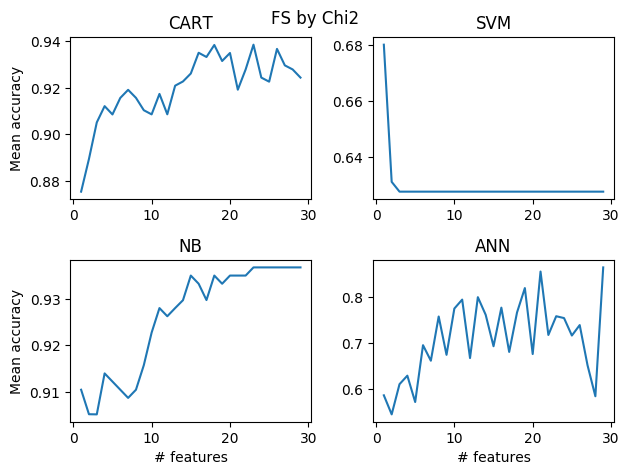
\includegraphics[width=\linewidth]{../plots/FS_by_Chi2.png}
  \caption{Performance by selecting features by Chi2}
  \label{fig:chi2}
\end{figure}

\begin{figure}[ht!]
  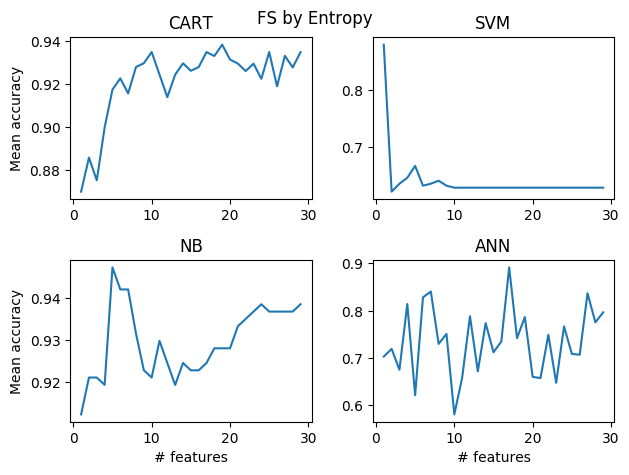
\includegraphics[width=\linewidth]{../plots/FS_by_Entropy.png}
  \caption{Performance by selecting features by Entropy}
  \label{fig:entropy}
\end{figure}

\begin{figure}[ht!]
  
\includegraphics[width=\linewidth]{../plots/RFS.png}
  \caption{Performance by selecting features by RFS}
  \label{fig:rfs}
\end{figure}

\section{Best features}

Could we tell which features contributes most to correct classification, how, why those

\section{Source of errors}

What can have caused faulty results, can our results be trusted?

\chapter{Discussion}

FNA is not that good compared to CNB \parencite{Topps2018}.

Let's discuss here

\chapter{Conclusion}

I guess this will be the last thing we write

\printbibliography[heading=bibintoc] % Print the bibliography (and make it appear in the table of contents)

\appendix

\chapter{Unnecessary Appended Material}

\end{document}
